\documentclass[UTF8]{ctexart}

\usepackage{fancyhdr}
\usepackage{titlesec}
\usepackage{geometry}
\geometry{a4paper,left=2cm,right=2cm,bottom=2.5cm,top=2.5cm}
\usepackage{graphicx}
\usepackage{epstopdf}
\usepackage{listings}
\usepackage{indentfirst}
\usepackage{multirow}
%\usepackage{time}
%\usepackage{times}
%\usepackage{datetime}
\usepackage{scrtime}
\graphicspath{ {figure/} } 

\pagestyle{fancy}
\lhead{SA18168163} 
\chead{可编程逻辑器件原理与应用} 
\rhead{杜沈达} 
\lfoot{} 
\cfoot{\thepage}
\rfoot{\em{Last Modified : \today \thistime}} 
\renewcommand{\headrulewidth}{0.4pt} 
\renewcommand{\footrulewidth}{0.4pt}

\newcommand{\major}{计算机应用技术}
\newcommand{\name}{杜沈达}
\newcommand{\stuid}{SA18168163}
\newcommand{\newdate}{2019年1月2日晚}
\newcommand{\loc}{一教实验室}
\newcommand{\course}{可编程逻辑器件原理与应用}
\newcommand{\grades}{}
\newcommand{\newtitle}{课程设计}

\makeatletter
\newcommand{\figcaption}{\def\@captype{figure}\caption}
\newcommand{\tabcaption}{\def\@captype{table}\caption}
\makeatother
\setlength{\parindent}{2.45em}

\begin{document}
\thispagestyle{empty}
	\begin{figure}[h]
		\begin{minipage}{0.6\linewidth}
			
\includegraphics[width=\linewidth]{head.jpg}
		\end{minipage}
		\hfill
		\begin{minipage}{.4\linewidth}
			\raggedleft
			\begin{tabular*}{.8\linewidth}{ll}
				专业: & \underline\major   \\
				姓名: & \underline\name    \\
				学号: & \underline\stuid   \\
				日期: & \underline\newdate \\
				地点: & \underline\loc
			\end{tabular*}
		\end{minipage}
	\end{figure}
	
	\begin{table}[!htbp]
		\centering
		\begin{tabular*}{\linewidth}{llllll}
			课程名称: & \underline\course   & 
			实验名称: & \underline\newtitle & 
			成绩:     & \underline\grades \\
		\end{tabular*}
	\end{table}

\titleformat*{\section}{\large\bfseries}
\titleformat*{\subsection}{\normalsize\bfseries}
\titleformat*{\subsubsection}{\normalsize}

\section{简介}
我的课程设计所用的DE2-115开发板,Quartus Prime17.0软件,DE2-115开发板外部有很多外围设备,能够保证足够的使用资源。使用Platform Designer制作需要功能的芯片,然后使用Quartus制作bdf文件,之后使用Nios II for Eclipse17.1软件编写程序,再将软硬件都烧录进目标板,也就实现了所需要的设计,设计的步骤如图1所示。
\begin{center}
	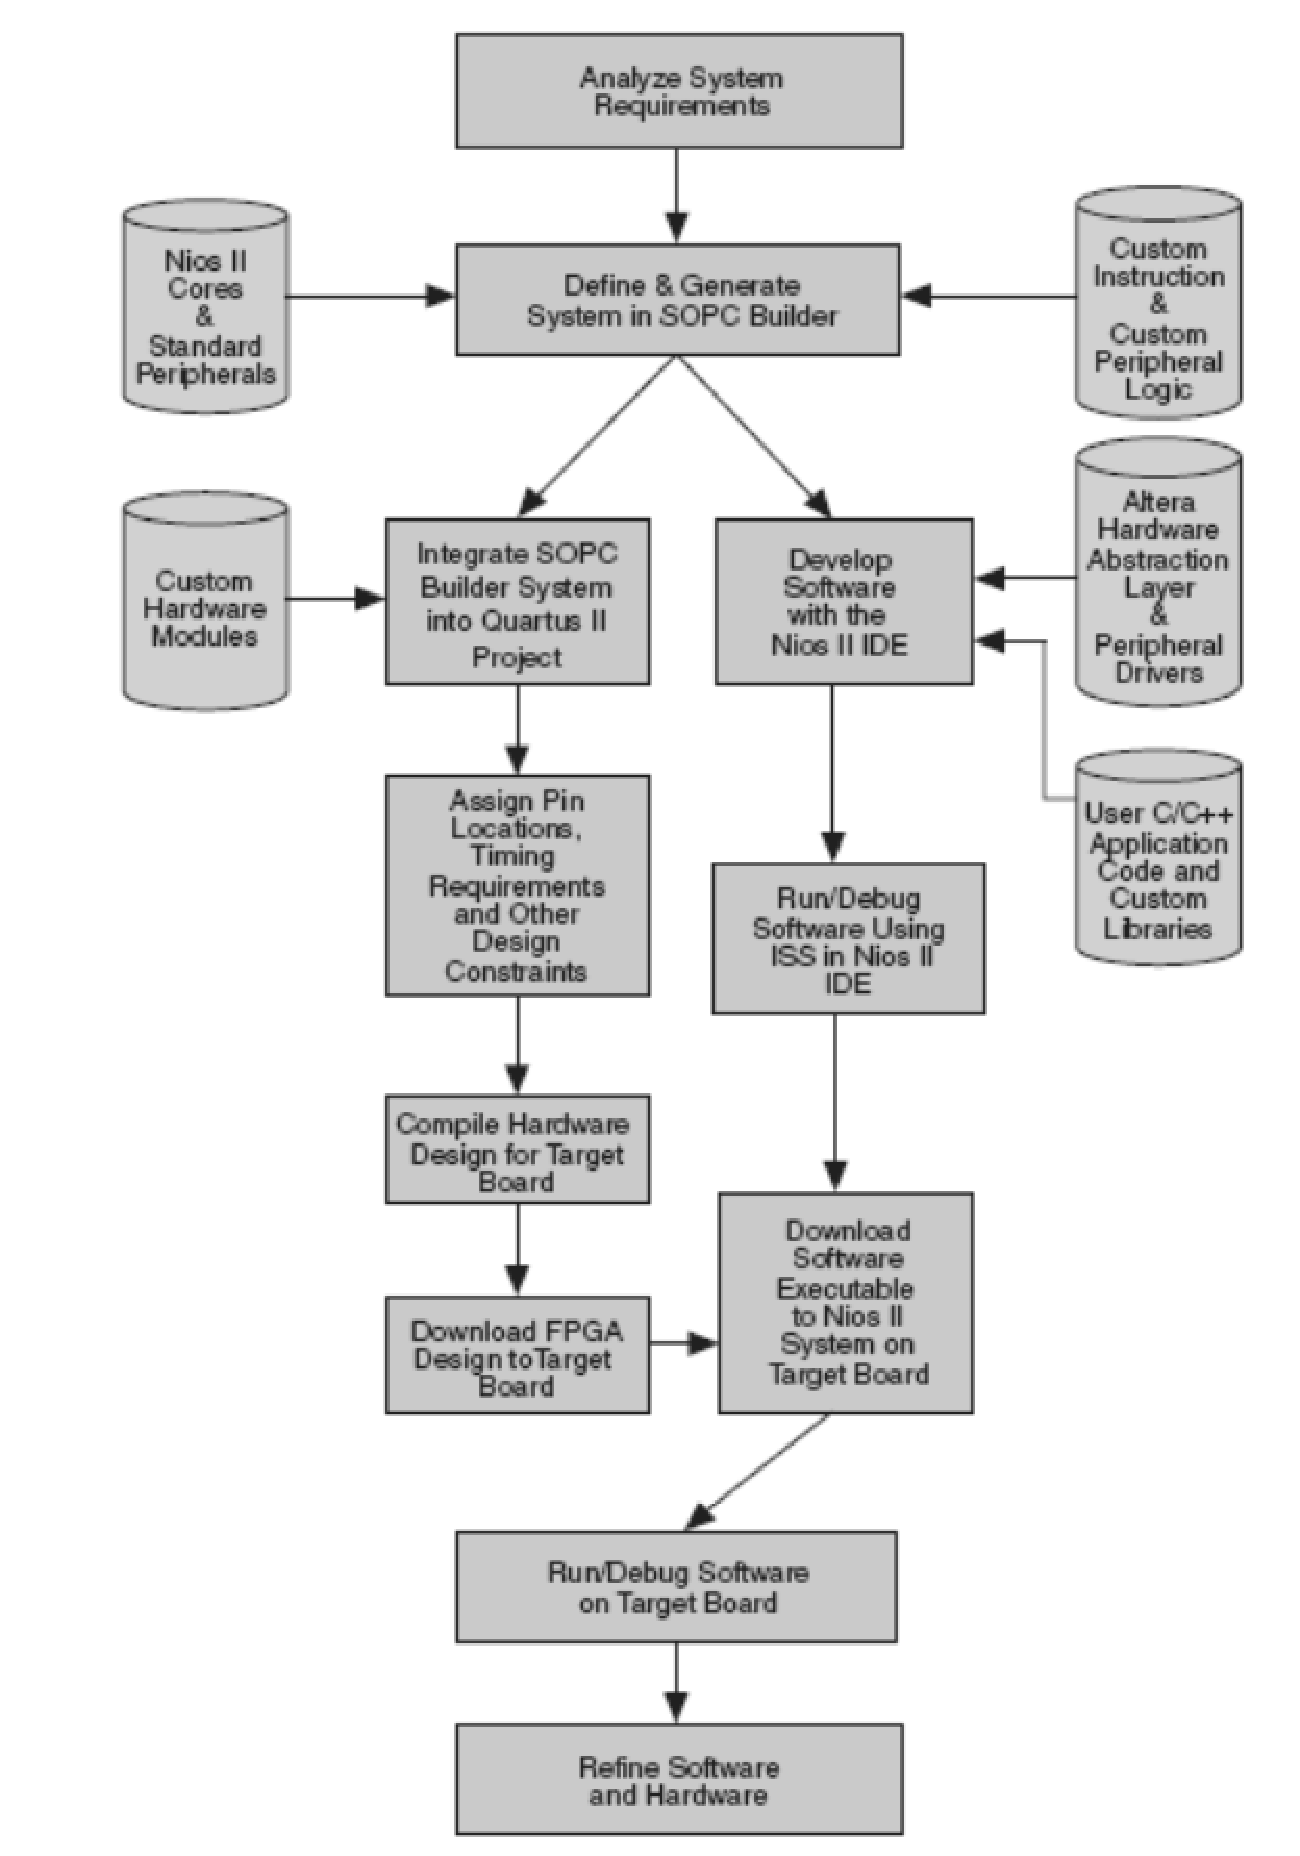
\includegraphics[width=14cm,height=15cm]{flow.eps}
	\figcaption{设计流程图}\label{flow}
\end{center}
\section{实现的功能}
\begin{enumerate}
	\item 实现8个绿色LED跑马灯;
	\item 实现数码管四位每秒自增一计时器;
	\item 实现数码管一位按下自增一计数器。
\end{enumerate}

\section{设计过程}
\subsection{NIOS设计}
如图2所示,先加入nios ii cpu,进行计算与控制,sdram作为随机存储器,uart用jtag口,作为调试口与PC通信,system id作为cpu标号,作为软硬件的交互,与时间戳一起判断是否匹配,使用一个1ms,32位的计时器,使用PIO口作为输出引脚,电平触发,对于LED采用8位PIO输出,数码管每个是7位输出,按钮1位输入。
	\begin{center}
		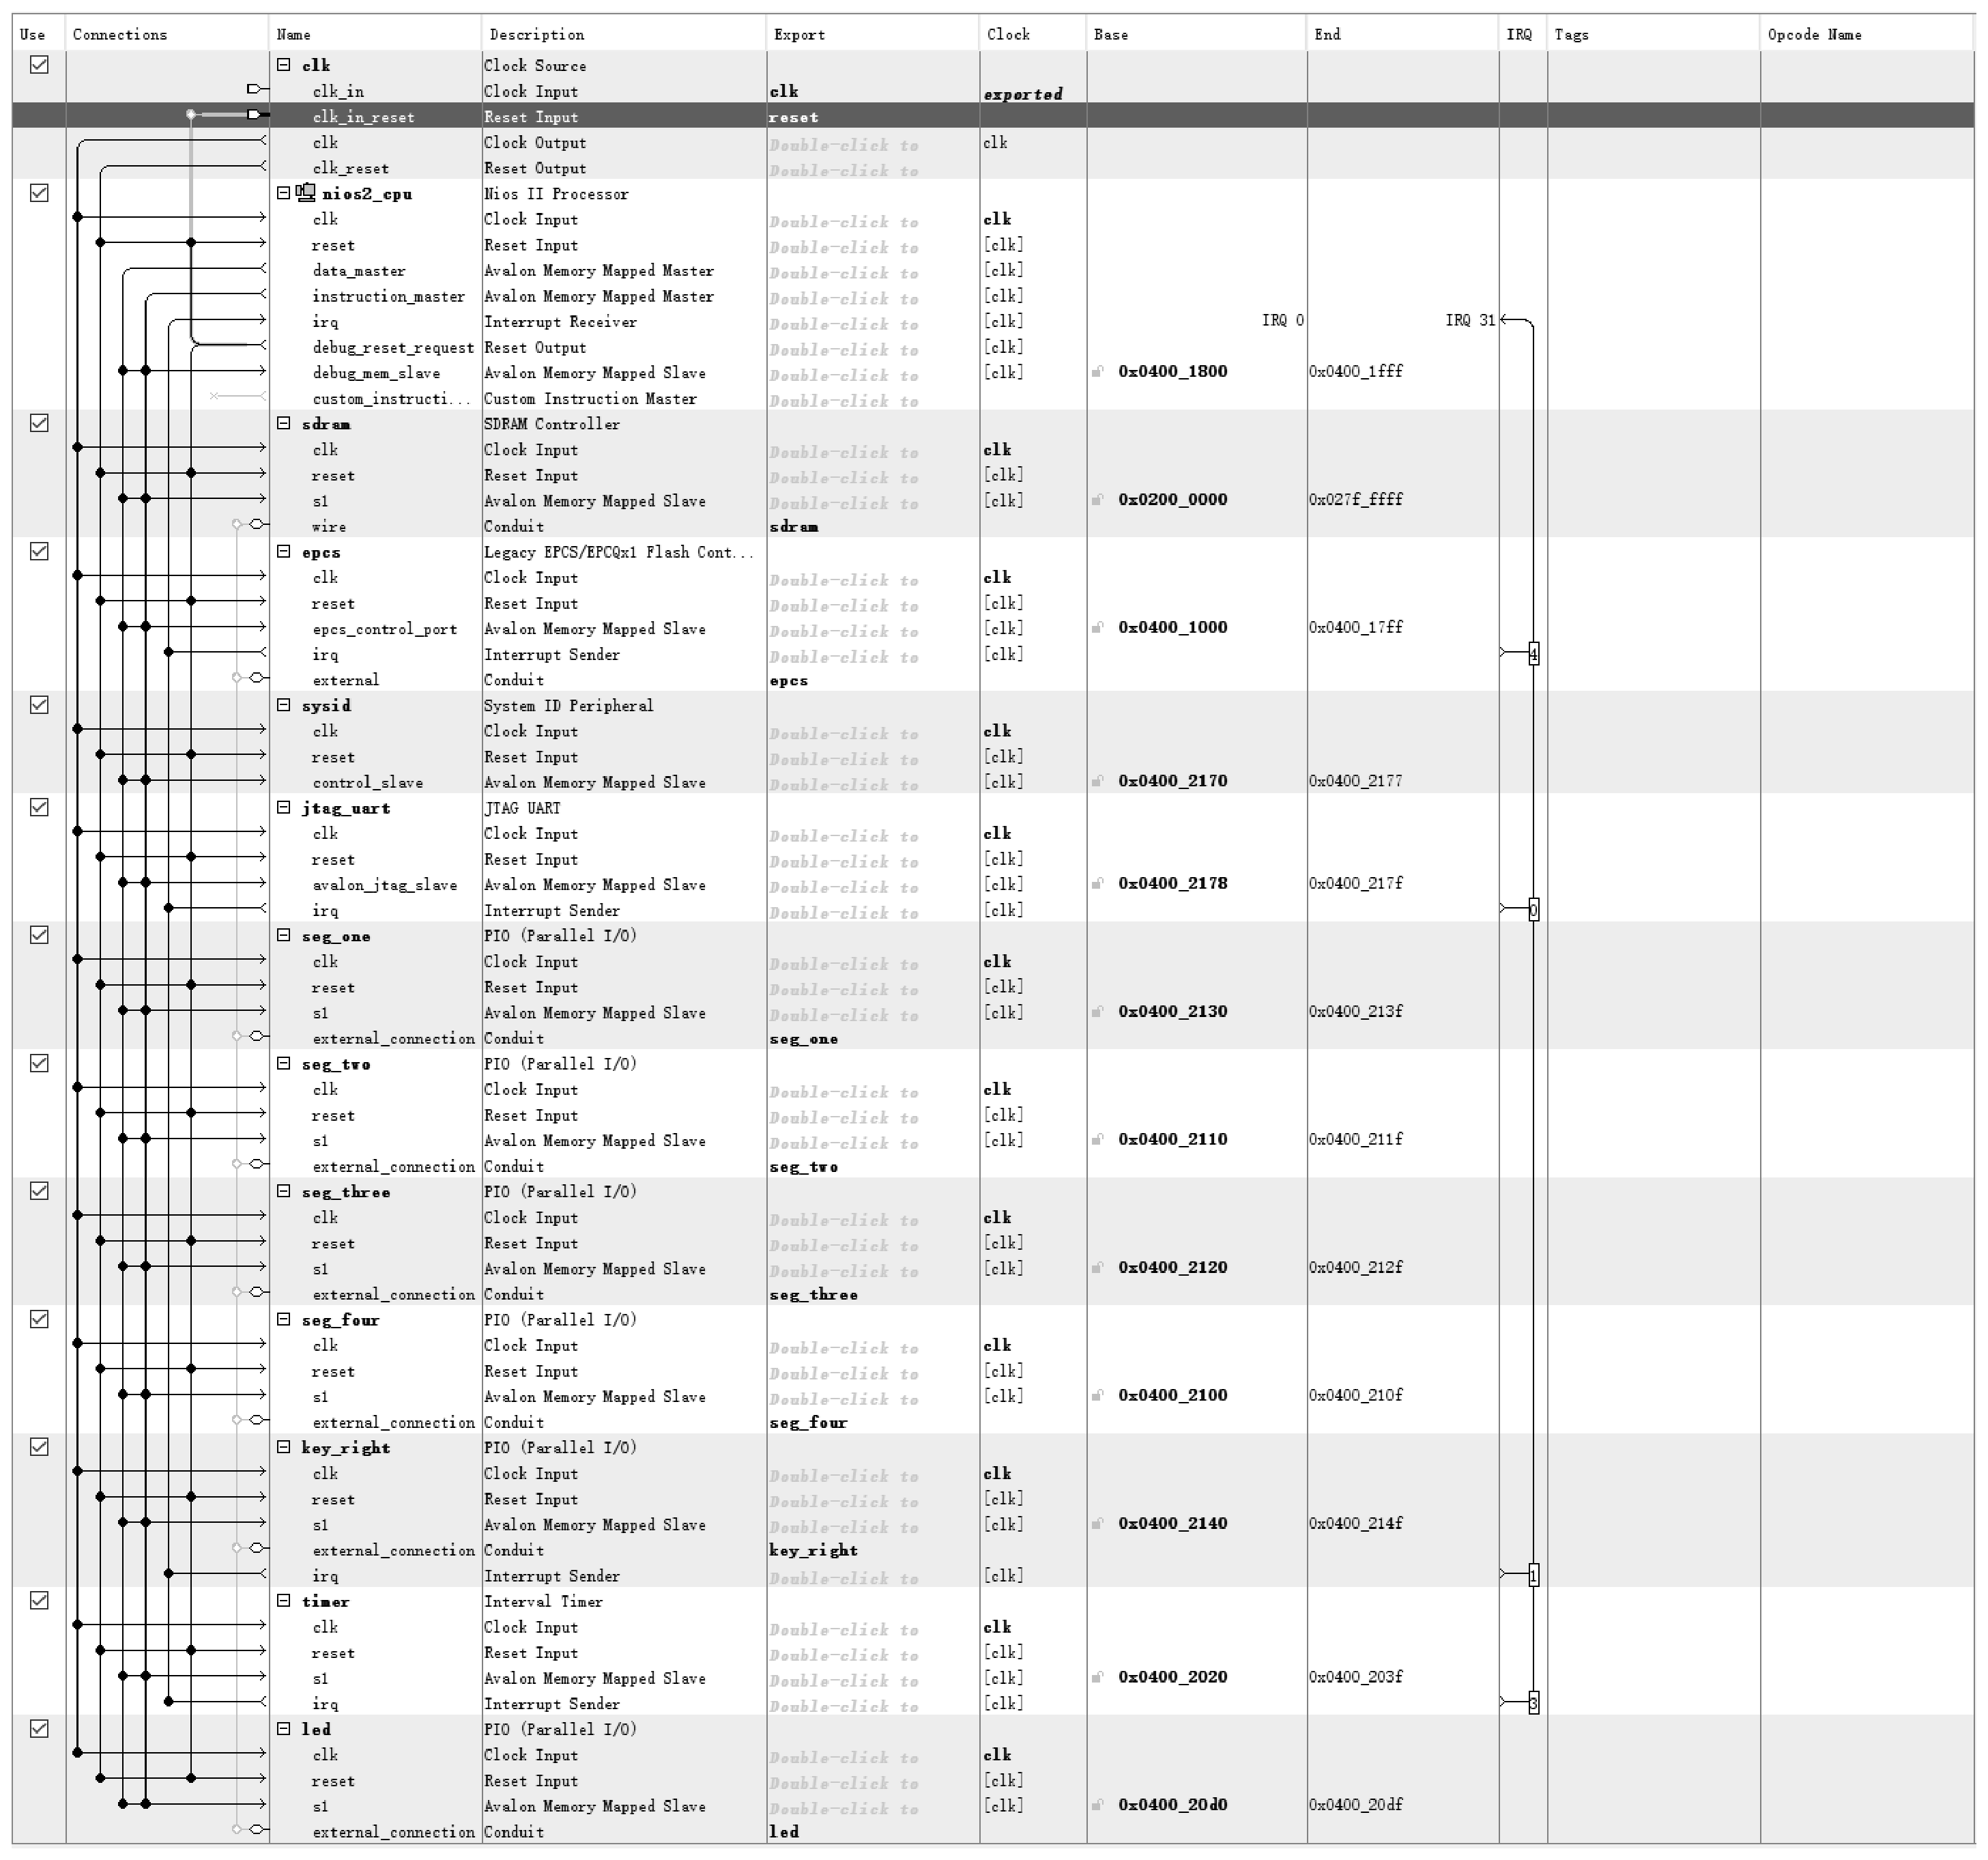
\includegraphics[width=16cm]{nios2.eps}
		\figcaption{NIOS II设计}\label{nios.eps}
	\end{center}

使用Avalon Memory Mapped内存映射总线,连接时钟,置位,读写地址与数据等信号,所有的时钟均采用50MHz,在按钮,epcs,jtag和定时器处设置断点,其中基地址由软件自动分配,完成后Generate成.bsf和Verilog语言的文件。
\begin{center}
	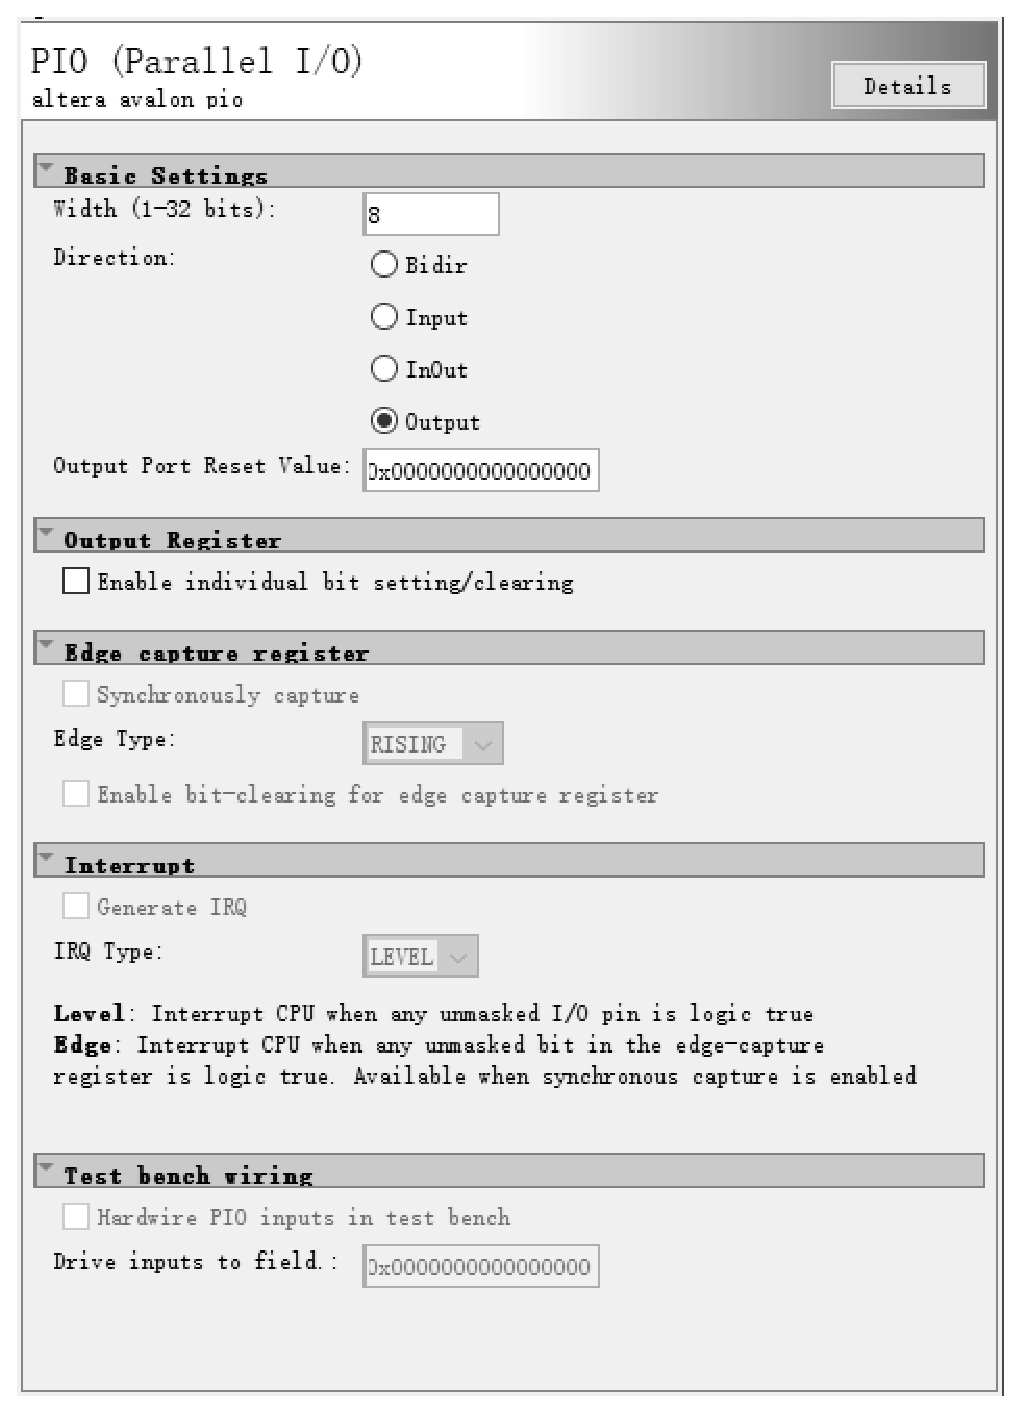
\includegraphics[width=8cm,height=10cm]{led.eps}
	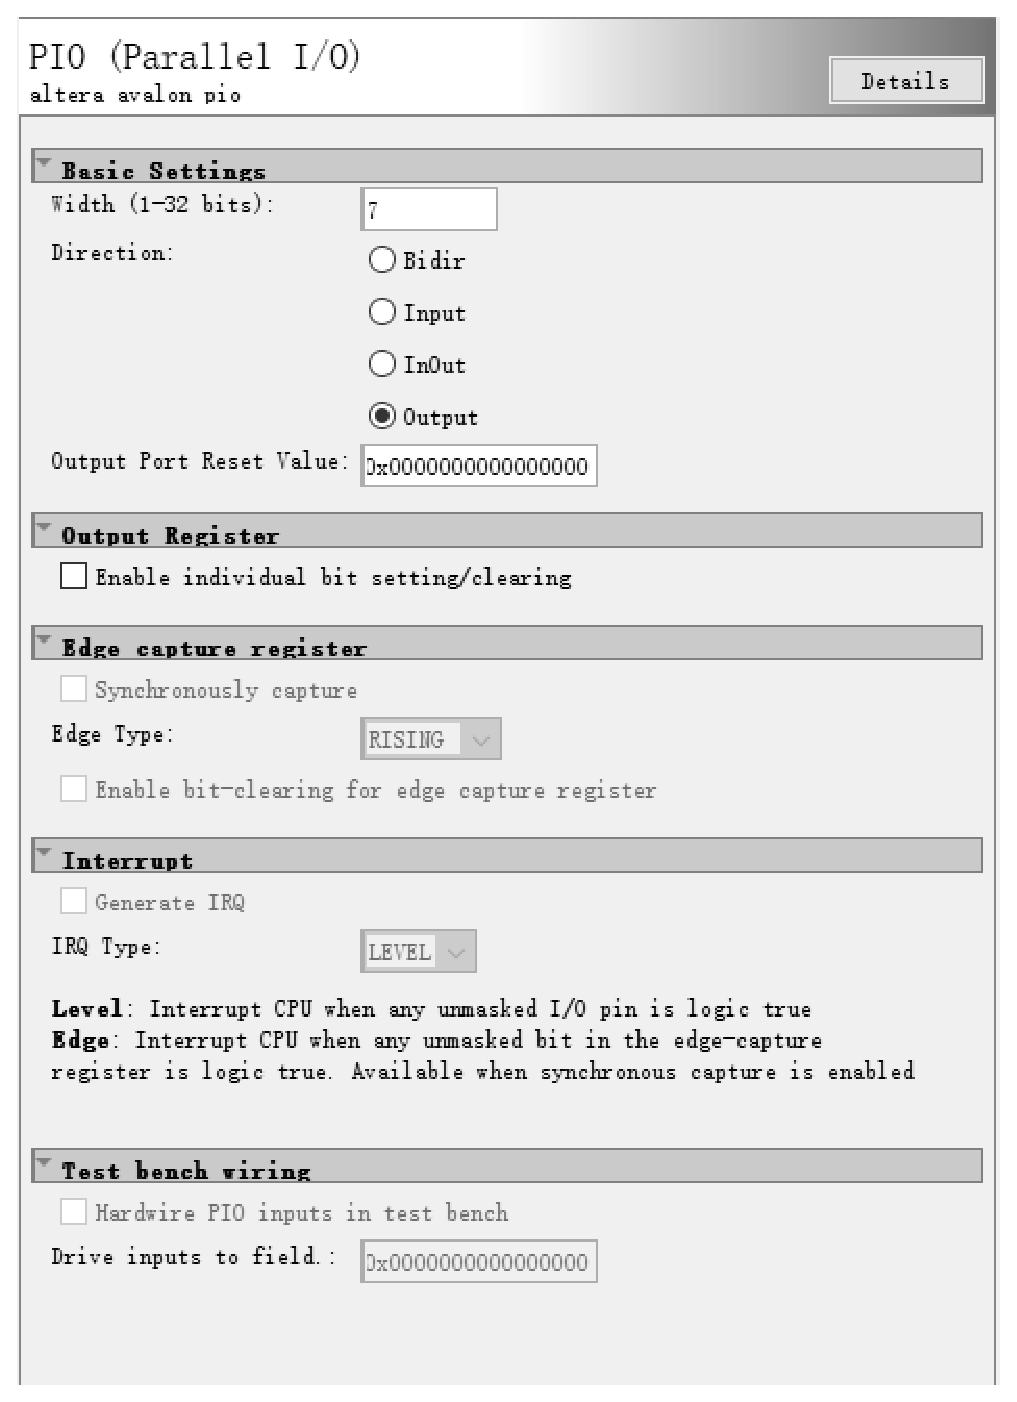
\includegraphics[width=8cm,height=10cm]{seg1.eps}
	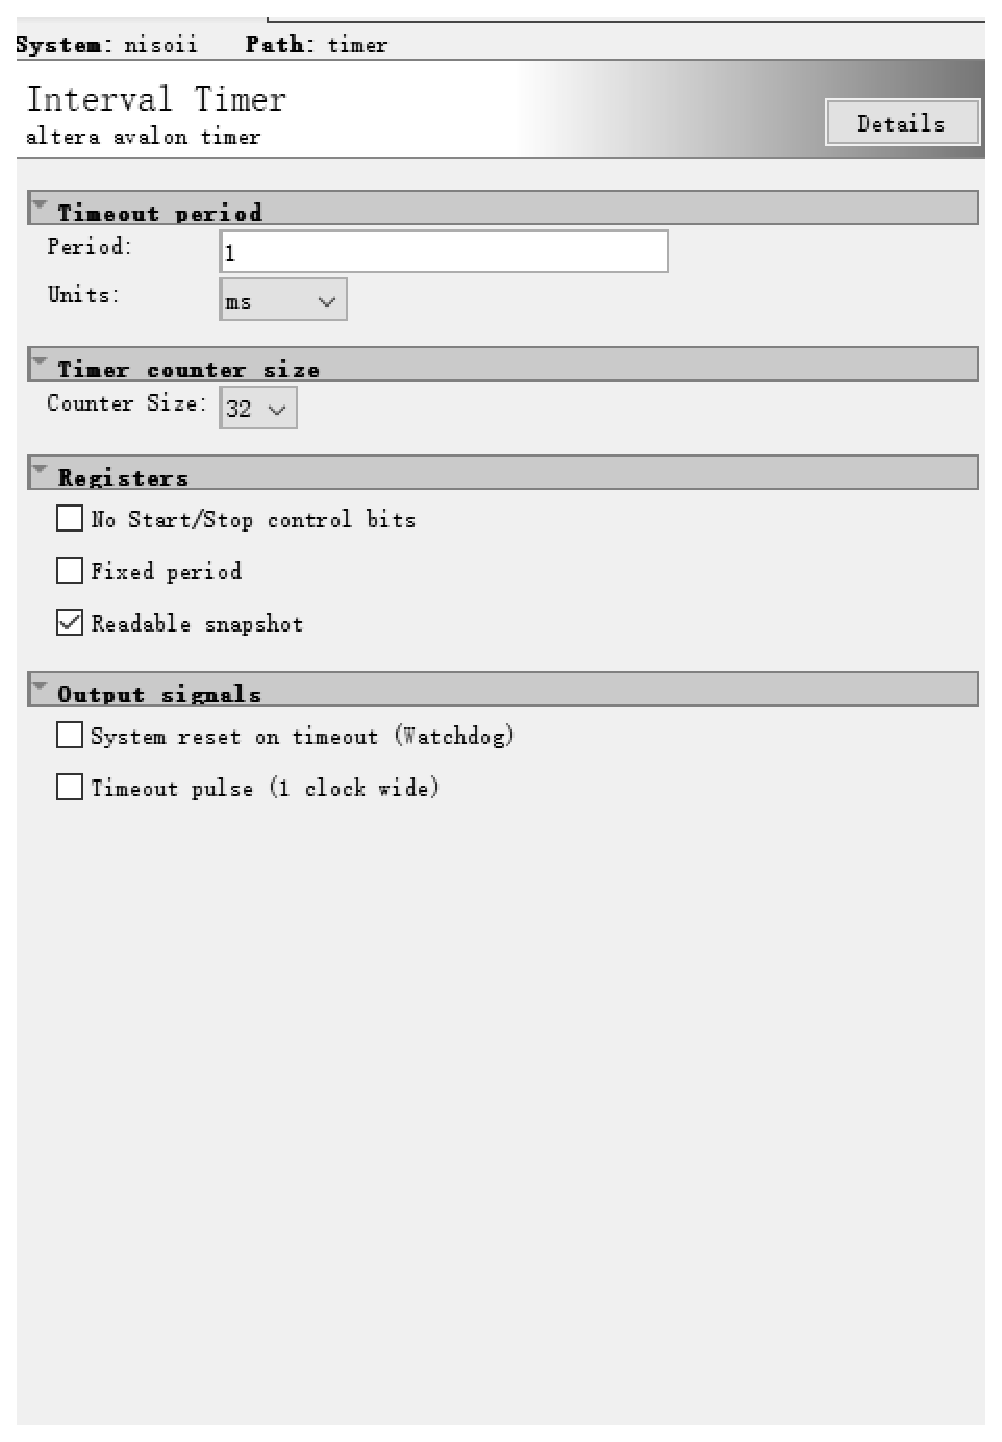
\includegraphics[width=8cm,height=10cm]{timer.eps}
	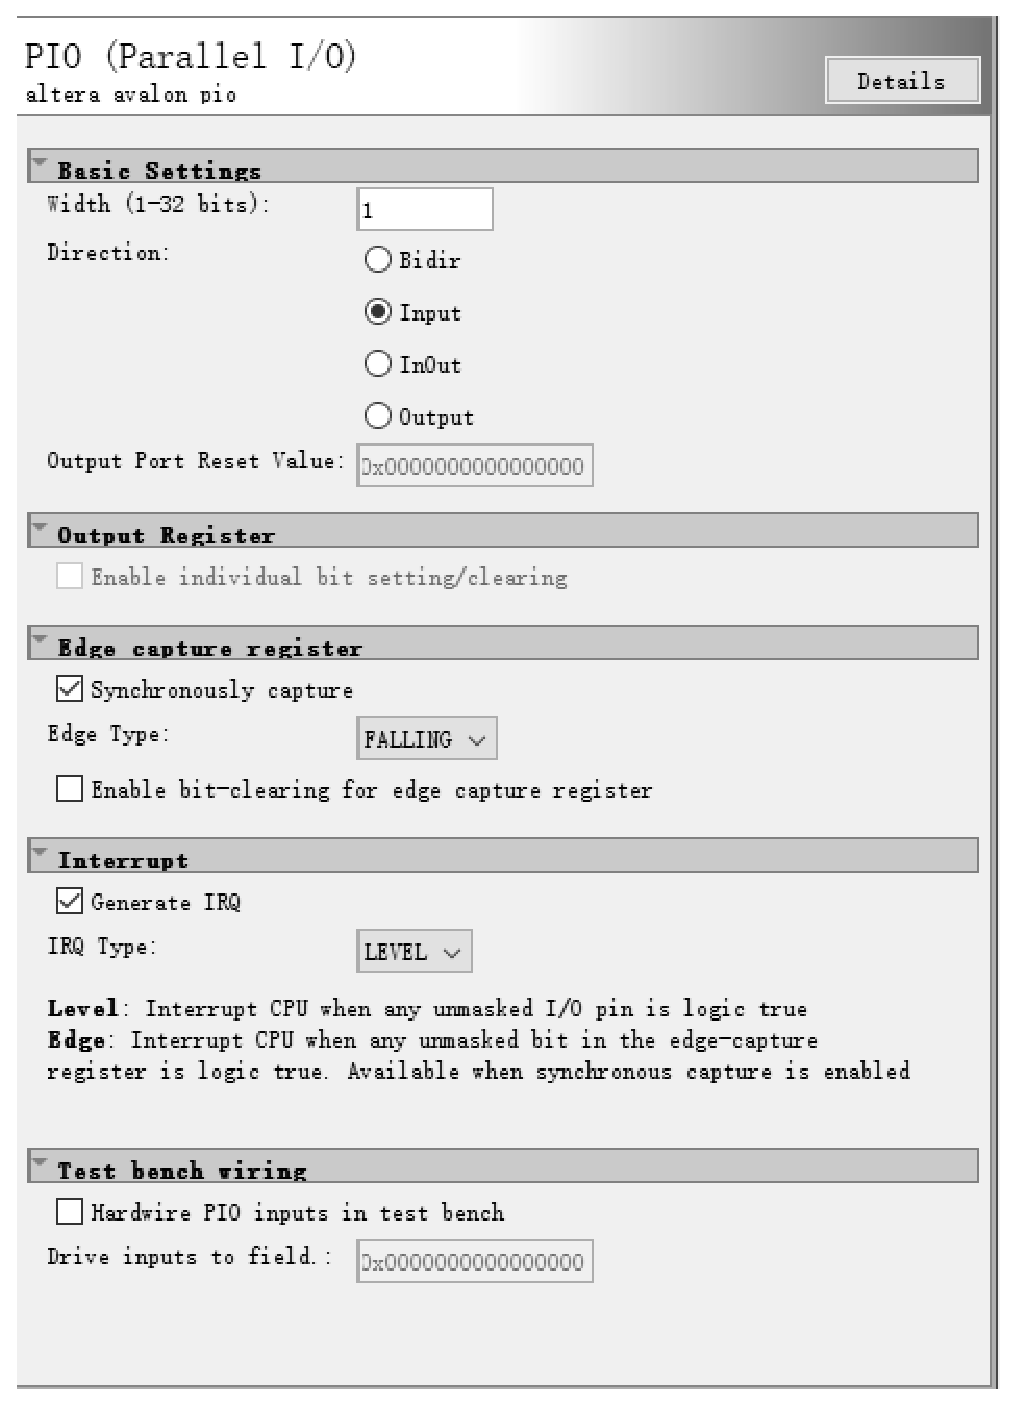
\includegraphics[width=8cm,height=10cm]{key.eps}
	\figcaption{各个连接部件参数}\label{detail.eps}
	(1)LED灯;(2)数码管;(3)定时器;(4)按钮
\end{center}	
\subsection{Quartus的.bdf文件绘制和引脚分配}
\subsubsection{.bdf文件绘制}
如图4所示,由inclk时钟信号经过PLL锁相环输入给nios ii cpu,将其reset位接vcc,即不置位,其余的管角均右键点击nios ii cpu点击Generate Pins for Symbol Port产生。
\begin{center}
	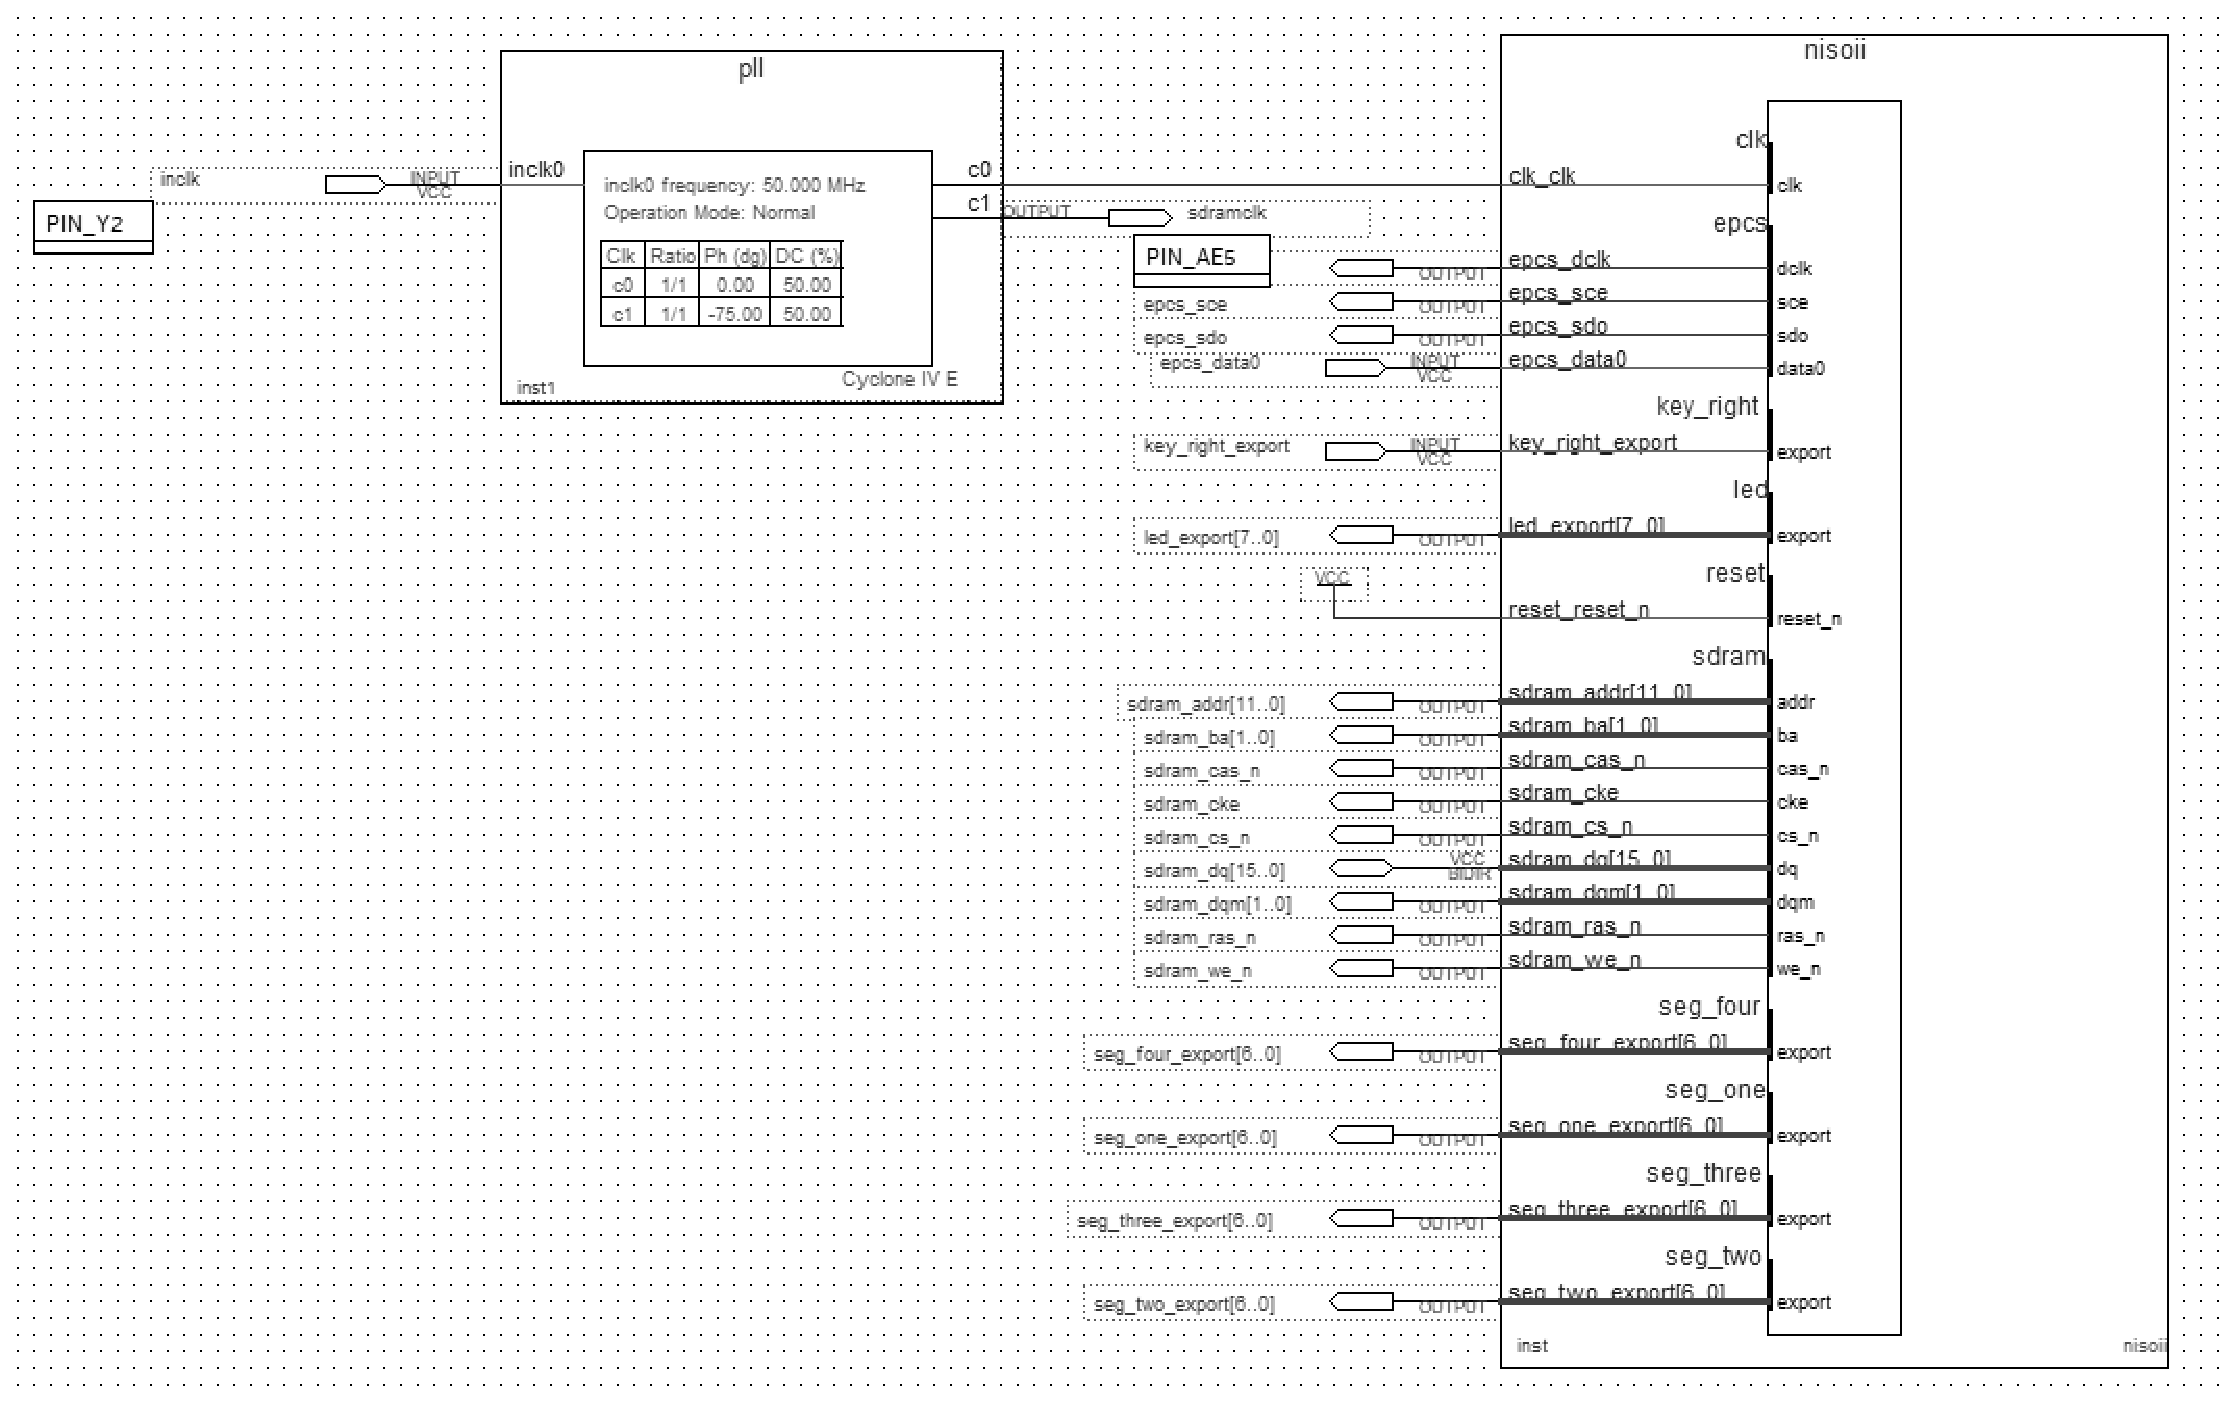
\includegraphics[width=16cm]{bdf.eps}
	\figcaption{bdf文件绘制}\label{bdf.eps}
\end{center}
\subsubsection{引脚分配}
参考DE2-115的用户手册,对于8个绿色LED灯的引脚分配如图5所示,
\begin{center}
	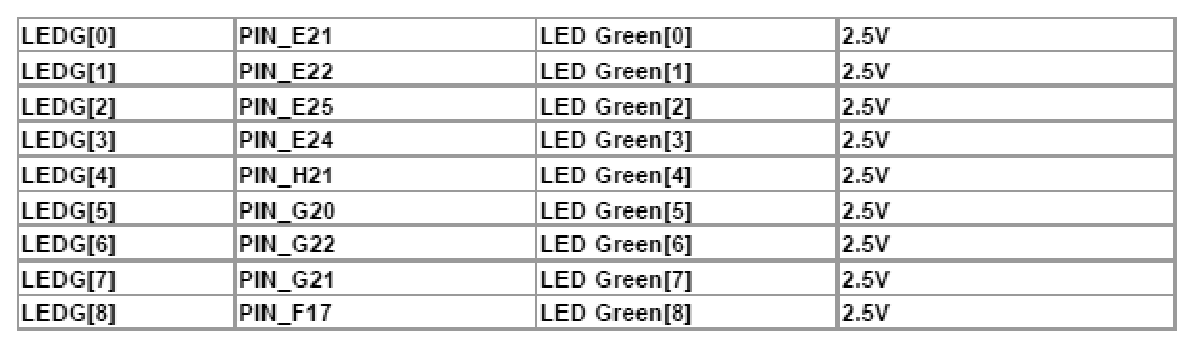
\includegraphics[width=8cm,height=4cm]{ledgpin.eps}
	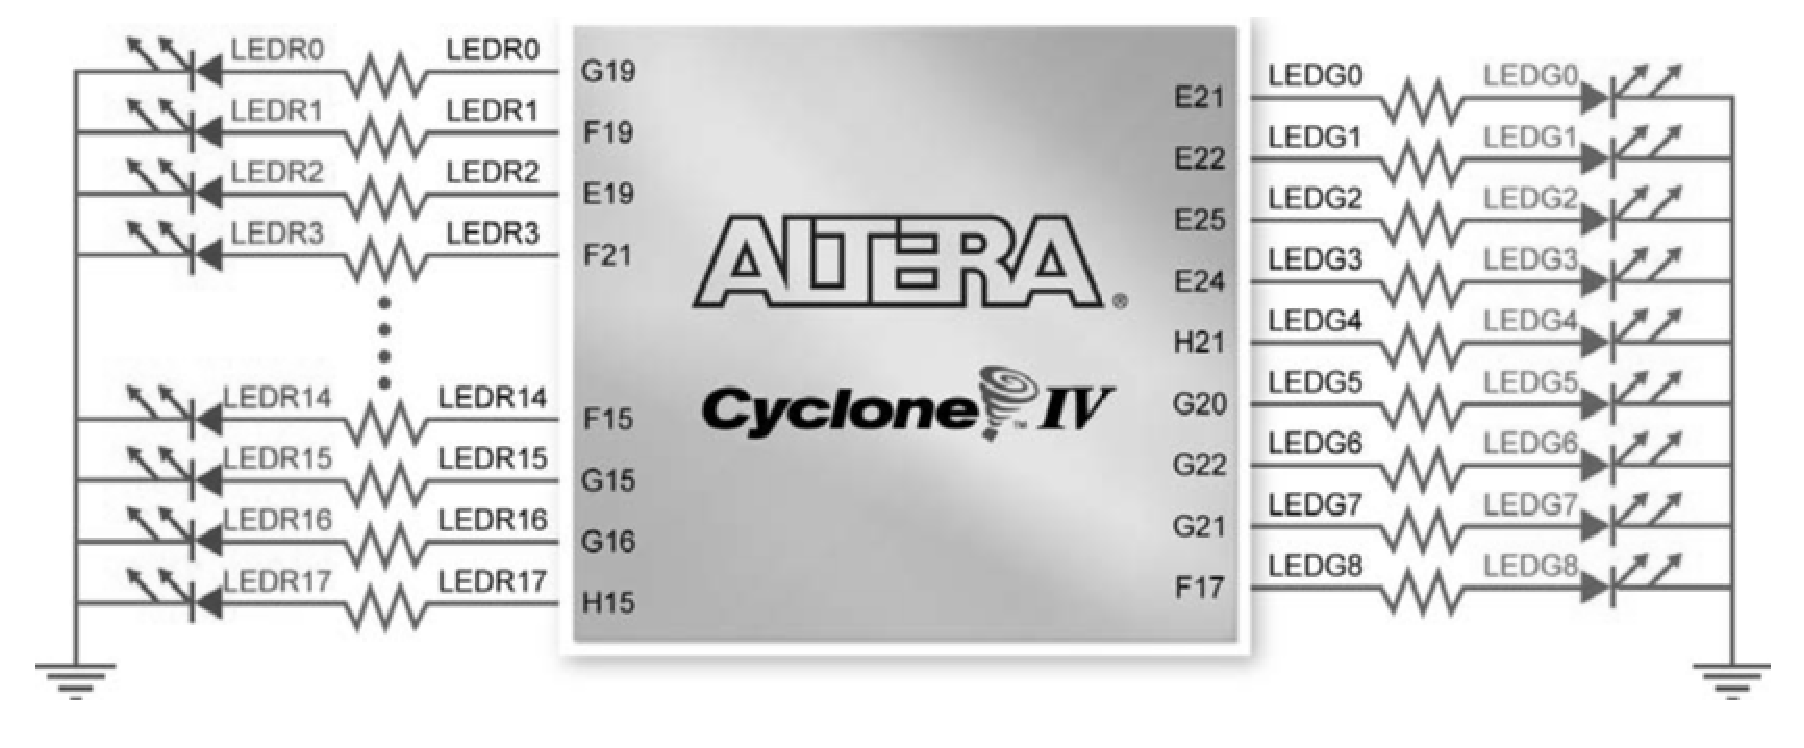
\includegraphics[width=8cm,height=4cm]{ledlianjie.eps}
	\figcaption{(1)LED管脚分配;(2)LED与FPGA连接}\label{leds.eps}
\end{center}

对于4个7段数码管的管脚分配可以由图6得到,DE2-115共有8个数码管,在这里只使用了四个,作为控制计数器和计时器使用。其中Key按钮和其他管脚的分配均可参考用户手册,或者从已经分配好的Excel文件中拷贝得到,这样更不容易出错,也大大减小了工作量。

最终的引脚分配如图7所示。
\begin{center}
	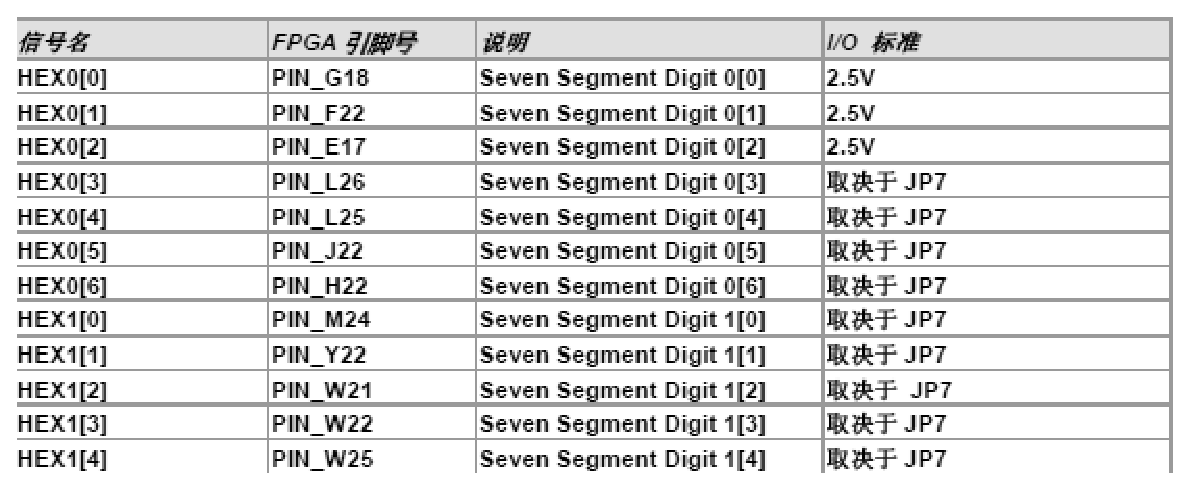
\includegraphics[width=8cm,height=5cm]{segpin.eps}
	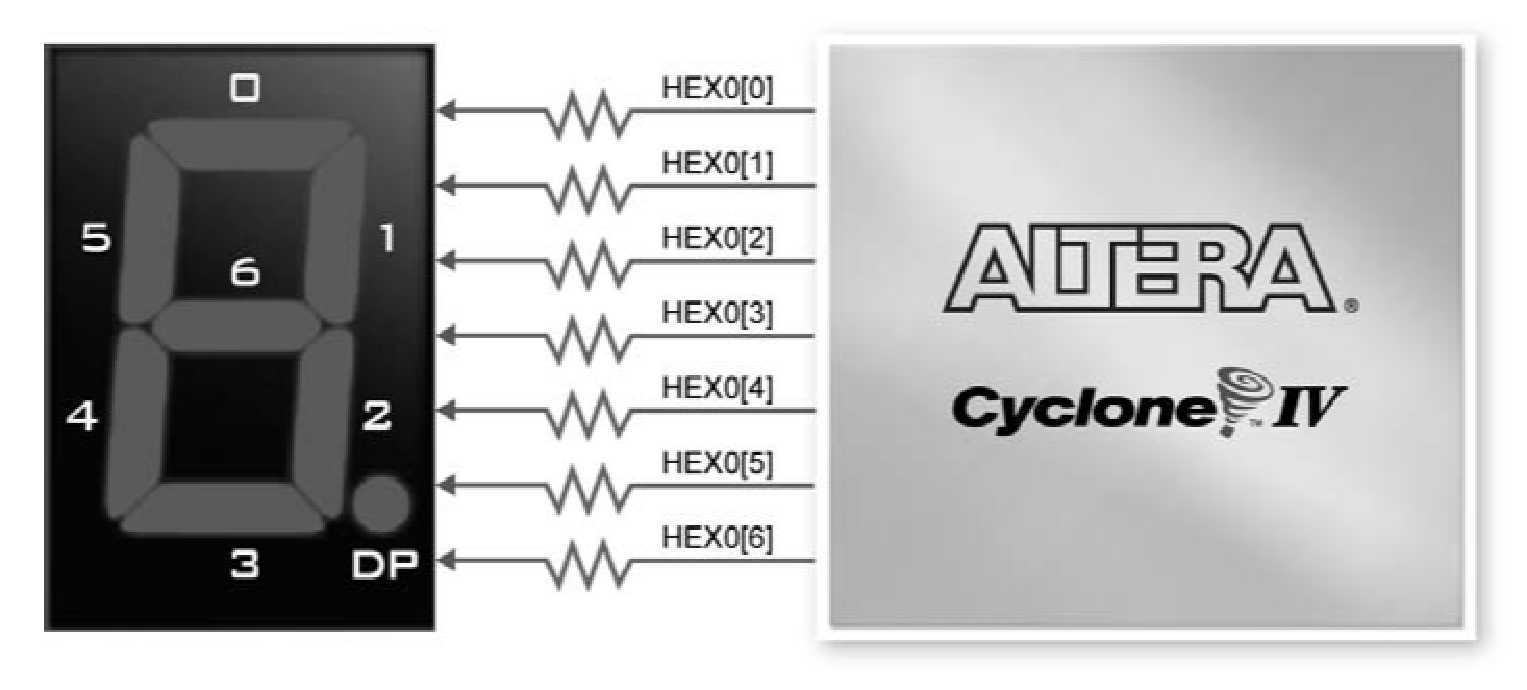
\includegraphics[width=8cm,height=5cm]{seglianjie.eps}
	\figcaption{(1)数码管管脚分配(截取部分);(2)数码管与FPGA连接}\label{segs.eps}
\end{center}
\begin{center}
		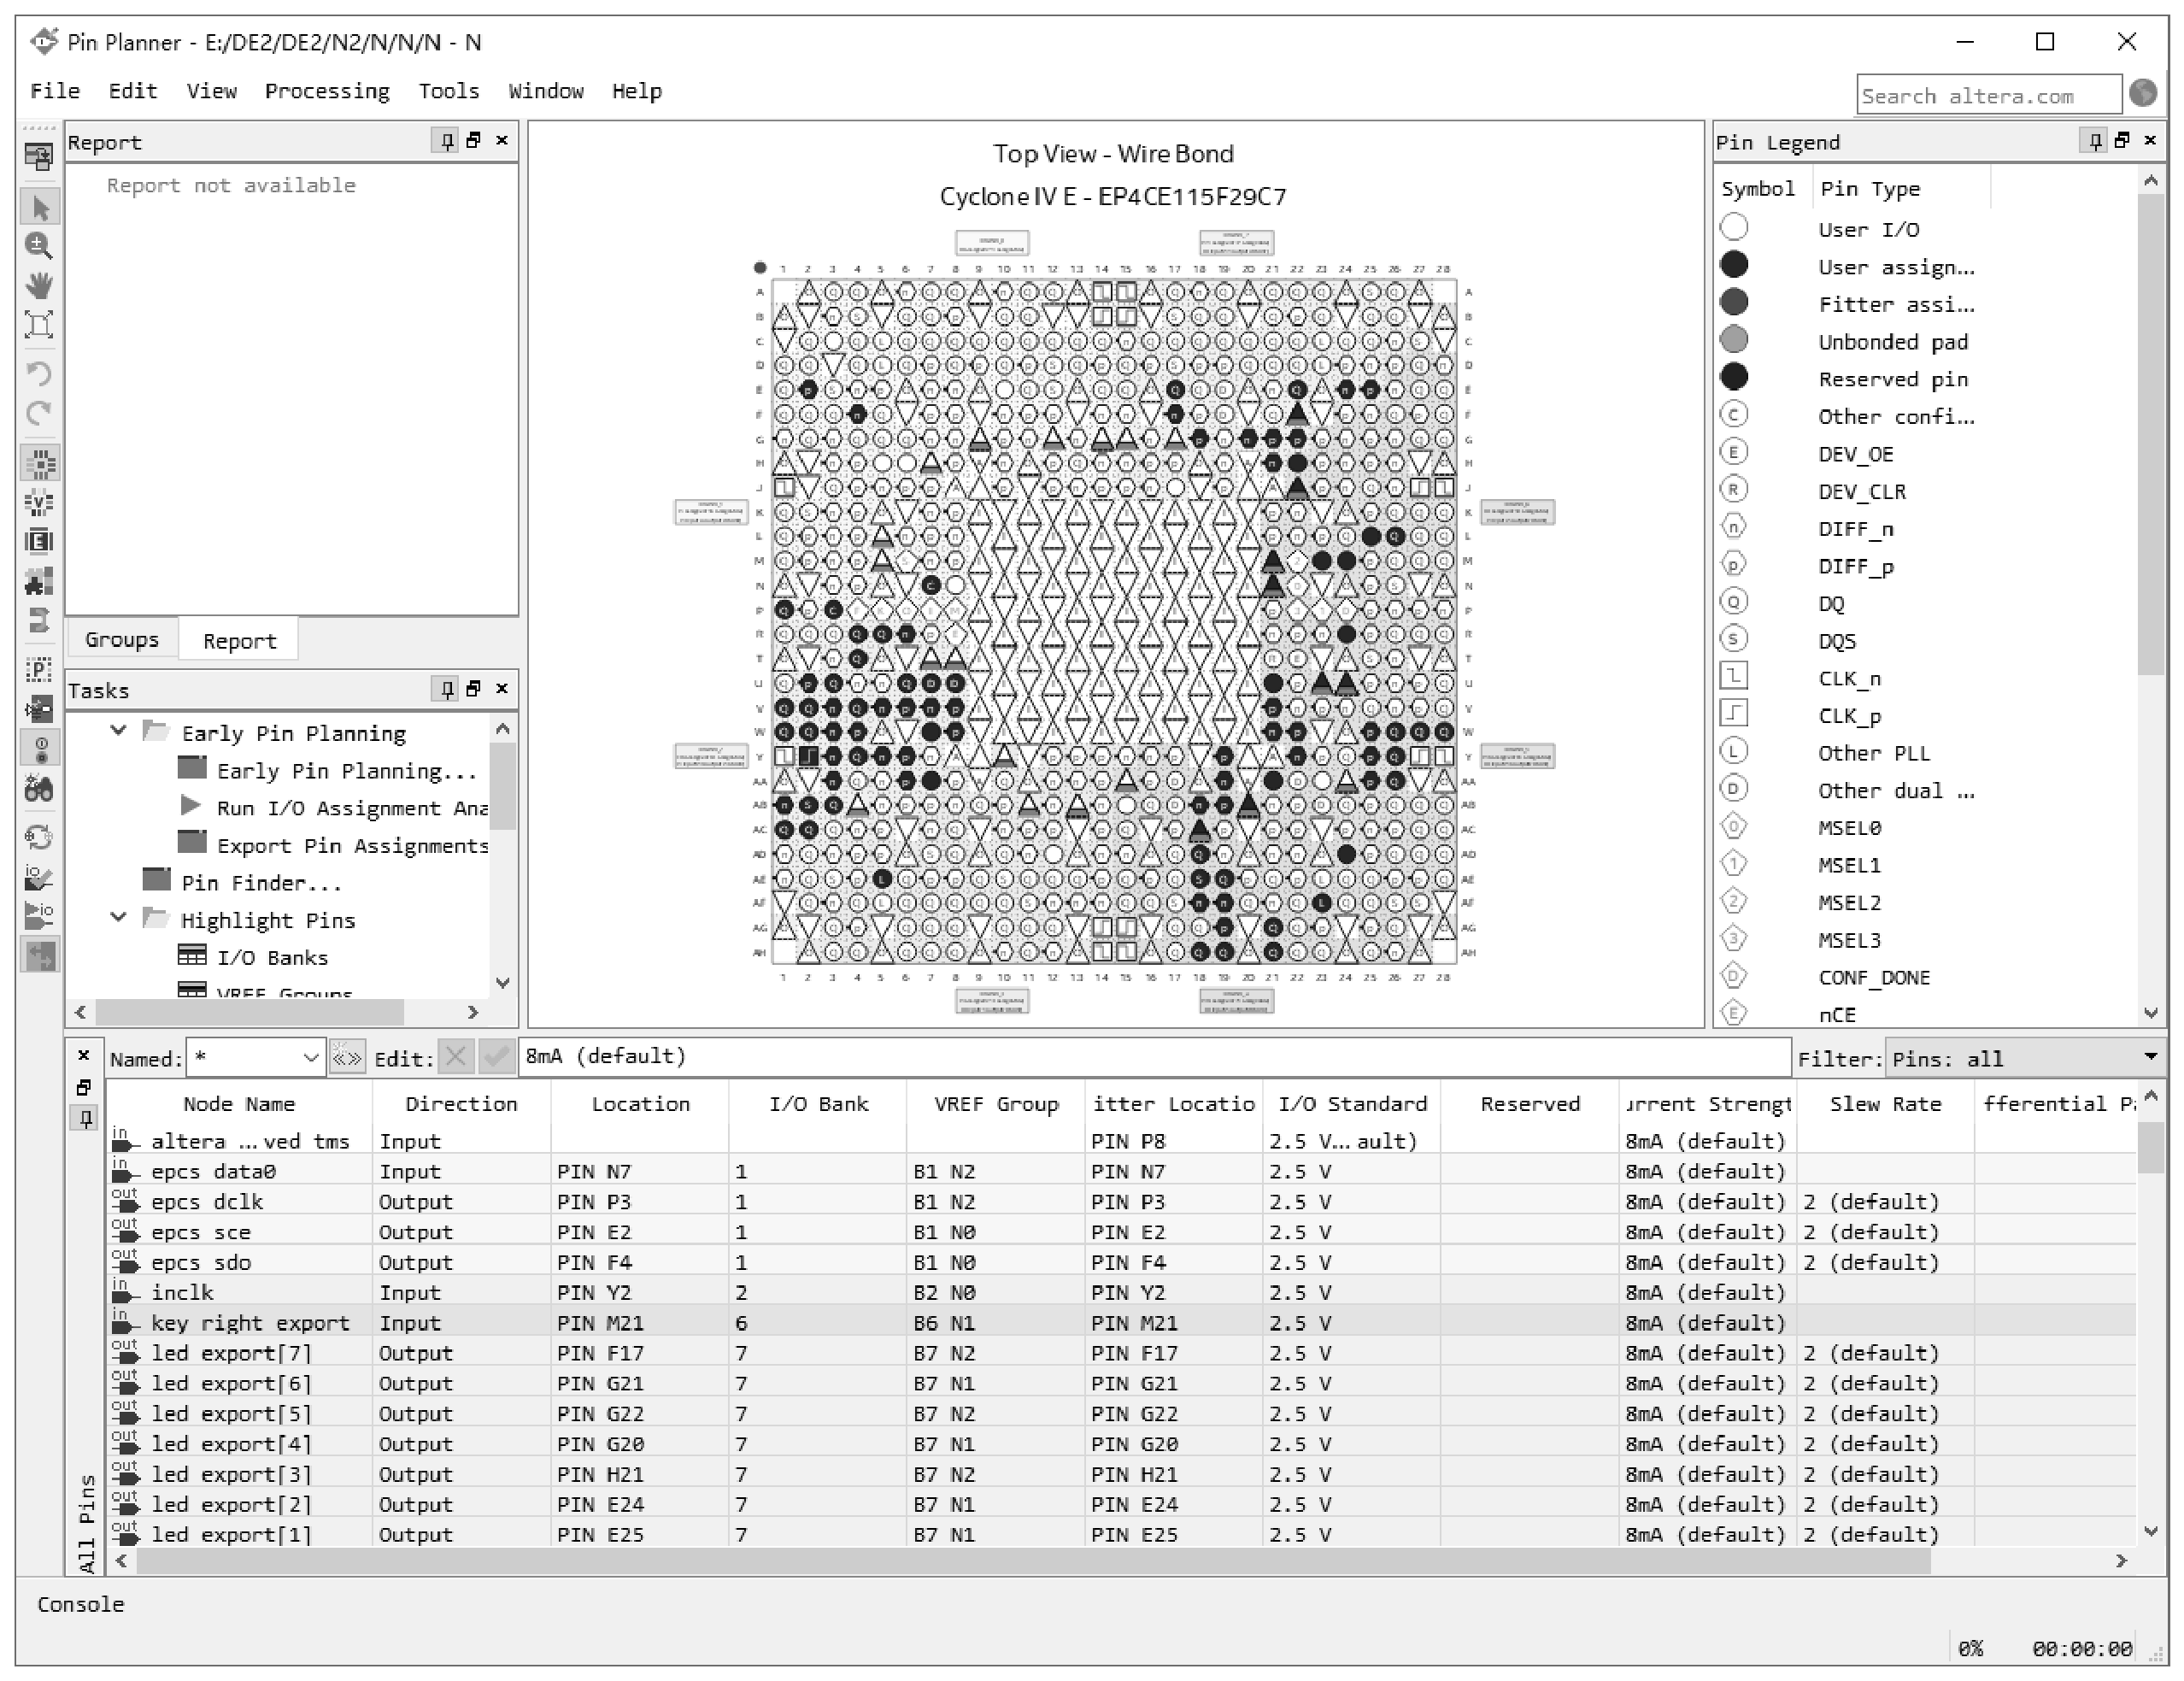
\includegraphics[width=16cm,height=16cm]{pinplaner.eps}
		\figcaption{最终的引脚分配}
\end{center}
\subsection{软件编写}
在完成了硬件部分的设计之后,要进行的就是软件的设计,从Platform Designer的Tool 里面打开NIOS II Software Build Tool for Eclipse,选择工作空间,新建一个NIOS Application and BSP from Template,选择sopc information文件。

之后进入软件的编写,首先定义一通用输入输出的结构体$PIO_STR$,包括基地址数据,方向,中断和边沿触发。又定义一定时器寄存器结构体。使用更好理解的$SEG_ONE$等代替数据所在的基地址,设置数码管的$1~9$显示数组。用Display函数进行显示输出,在主函数中写一个死循环,数码管每秒加1,直到碰到按钮进行中断,令对应的控制的数码管加1,LED灯的控制完全自己进行。也就是每秒LED的寄存器变化一次,下一个灯开始亮,如此循环往复。
具体的程序如下:
\lstinputlisting[language={C++},
numbers=left, numberstyle={\normalsize },	commentstyle=\color{red!50!green!50!blue!50}, 
frame=shadowbox, rulesepcolor=\color{red!20!green!20!blue!20}]
{code/n.c}

\end{document}

